\hspace{1.5cm}
A Calibração Radiométrica é aplicada para imagens do tipo ASTER, AVHRR, MSS, QuickBird, TM and TIMS, com vista a realizar a técnicas de correções atmosférica. As imagens adquiridas foram do Landsat 5 TM, que foram calibradas pelo \textbf{\textit{Landsat TM Calibration}}, do programa Envi 4.7. A calibração se deu em todas as Bandas baixadas, excetuando a banda 6, do anos de 1999 e 2011. Processo foi realizado individualmente, para as 12 (dozes) bandas.

\hspace{1.5cm}
O processo de calibração ocorreu da seguinte forma:
\begin{itemize}
\item \textbf{Basic Tools}
\begin{itemize}
\item \textbf{Preprocessing  $\rightarrow$  Calibration Utilities  $\rightarrow$  Landsat TM}.\\
\end{itemize}
\begin{figure}[h!]
\centering
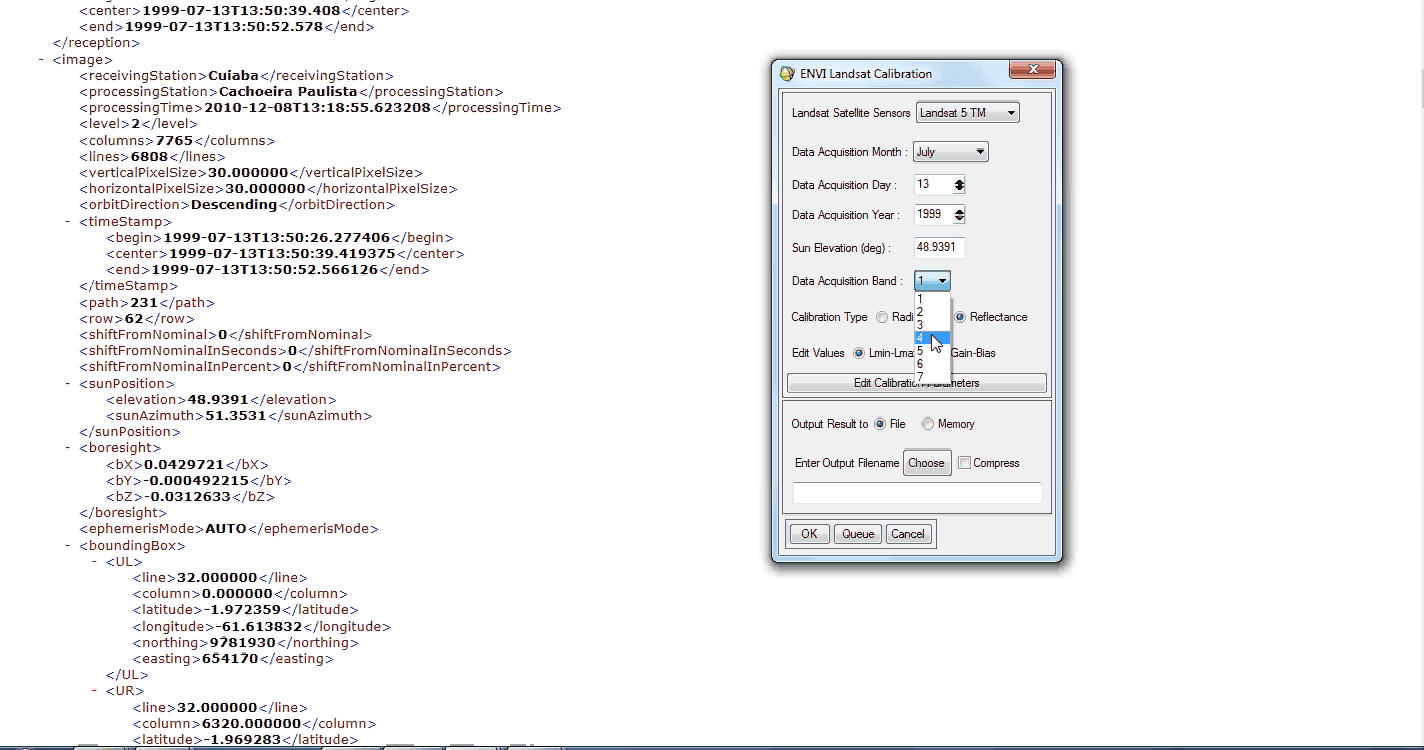
\includegraphics[scale=0.3]{imagens/calibracao03.png}
\caption{Configuração para calibração das imagens.}
\label{calibracao03}
\end{figure}

\end{itemize}
\hspace{1.5cm} Na janela \textbf{\textit{TM Calibration Parameters}} é selecionado o tipo de satélite, no nosso caso \textit{Landsat 5}; Mês de aquisição da imagem, no primeiro conjunto  08 e no segundo 10; dia de aquisição da imagem, no primeiro conjunto  13 e no segundo 23; Ano de aquisição da imagem, no primeiro conjunto  1999 e no segundo 2011;e Sun Elevation, em cada banda (figura ) foi adquirido um grau diferente, dentro de um arquivo XML (figura \ref{calibracao03}).
Após o procedimento escolhe o tipo de saída do resultado: \textbf{Arquivo} e salva.